This concluding chapter presents a follow-up to the analytical-empirical results previously discussed, offering an improved architectural design that is more scalable and capable of serving a greater number of customers.
As with the queueing network analysed throughout the report, the same theoretical analysis procedure will be employed to confirm the enhanced performance of the proposed architecture.

\section{Queueing network components}

The proposed architecture is illustrated below.
As the initial analysis of the first queueing network indicated that the database station was the bottleneck, our solution proposes a horizontal scaling of that component, with the introduction of a second replica.

\begin{center}
	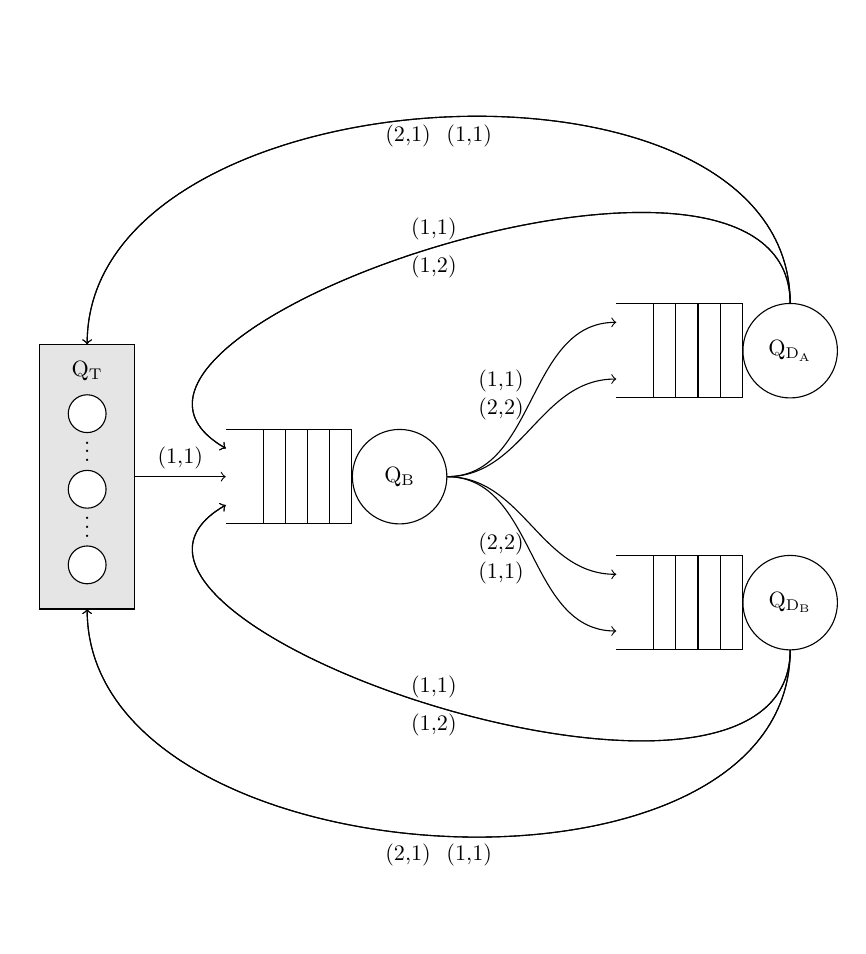
\begin{tikzpicture}[scale=0.8, transform shape]
		\tikzstyle{thinking_station} = [rectangle, draw, minimum height=4.2cm, minimum width=1.5cm, fill=gray!20, align=left]
		\tikzstyle{circle_node} = [circle, draw, fill=white, minimum size=6mm, inner sep=0pt]
		\tikzstyle{queue} = [circle, draw, minimum size=1cm, text centered, inner sep=0pt]
	
		% Thinking station
		\node (QT) [thinking_station] at (0,0) {};
		\node at (0,1.68) {Q\textsubscript{T}};
		% Users belonging to the closed loop
		\node[circle_node] at (0, 1) {};
		\node at (0, 0.5) {$\vdots$};
		\node[circle_node] at (0, -0.2) {};
		\node at (0, -0.7) {$\vdots$};
		\node[circle_node] at (0, -1.4) {};
	
		% Backend station
		% Queue
		\draw (2.2,0.75) -- ++(2cm,0) -- ++(0,-1.5cm) -- ++(-2cm,0);
		\foreach \i in {1,...,4}
		\draw (4.2cm-\i*10pt,0.75) -- +(0,-1.5cm);
		% Service room
		\draw (4.96,-0.00cm) circle [radius=0.75cm];
		% Label service time
		\node at (4.96,-0.00cm) {Q\textsubscript{B}};
	
		% Database station 1
		% Queue
		\draw (8.4,2.75) -- ++(2cm,0) -- ++(0,-1.5cm) -- ++(-2cm,0);
		\foreach \i in {1,...,4}
		\draw (10.4cm-\i*10pt,2.75) -- +(0,-1.5cm);
		% Service room
		\draw (11.160,2.00cm) circle [radius=0.75cm];
		% Label service time
		\node at (11.160,2.00cm) {Q\textsubscript{D\textsubscript{A}}};
	
		% Database station 2
		% Queue
		\draw (8.4,-1.25) -- ++(2cm,0) -- ++(0,-1.5cm) -- ++(-2cm,0);
		\foreach \i in {1,...,4}
		\draw (10.4cm-\i*10pt,-1.25) -- +(0,-1.5cm);
		% Service room
		\draw (11.160,-2.00cm) circle [radius=0.75cm];
		% Label service time
		\node at (11.160,-2.00cm) {Q\textsubscript{D\textsubscript{B}}};
	
		\draw[->]	(QT) to[out=0,in=180] node[above]	{(1,1)} (2.2,0);
		\draw[->]	(5.71,0) to[out=0,in=180] node[above left] {(1,1)} (8.4,2.45);
		\draw[->]	(5.71,0) to[out=0,in=180] node[above left] {(2,2)} (8.4,1.55);
		\draw[->]	(5.71,0) to[out=0,in=180] node[below left] {(1,1)} (8.4,-2.45);
		\draw[->]	(5.71,0) to[out=0,in=180] node[below left] {(2,2)} (8.4,-1.55);
		\draw[->]	(11.160,2.75) to[out=90,in=150] node[above] {(1,1)} (2.2,0.45);
		\draw[->]	(11.160,2.75) to[out=90,in=150] node[below] {(1,2)} (2.2,0.45);
		\draw[->]	(11.160,-2.75) to[out=-90,in=-150] node[above] {(1,1)} (2.2,-0.45);
		\draw[->]	(11.160,-2.75) to[out=-90,in=-150] node[below] {(1,2)} (2.2,-0.45);
		\draw[->]	(11.160,2.75) to[out=90,in=90] node[below left] {(2,1)} (0,2.1);
		\draw[->]	(11.160,2.75) to[out=90,in=90] node[below right] {(1,1)} (0,2.1);
		\draw[->]	(11.160,-2.75) to[out=-90,in=-90] node[below left] {(2,1)} (0,-2.1);
		\draw[->]	(11.160,-2.75) to[out=-90,in=-90] node[below right] {(1,1)} (0,-2.1);
	\end{tikzpicture}
\end{center}

\section{Q.N. theoretical analysis}

\subsection{Traffic equations}

The system's traffic equations are presented below. 
As previously stated in the initial queueing network analysis, these values also represent the relative visit ratios ($\overline{V}_{i}$).

\[
	\begin{array}{c}
		\begin{bmatrix}
		p_{T1B1} \\
		p_{B1D_{A}1} \\
		p_{B1D_{B}1} \\
		p_{B2D_{A}2} \\
		p_{B2D_{B}2} \\
		p_{D_{A}1B1} \\
		p_{D_{A}1B2} \\
		p_{D_{A}1T1} \\
		p_{D_{A}2T1} \\
		p_{D_{B}1B1} \\
		p_{D_{B}1B2} \\
		p_{D_{B}1T1} \\
		p_{D_{B}2T1} \\
		\end{bmatrix}
		=
		\begin{pmatrix}
		1.0 \\
		0.5 \\
		0.5 \\
		0.5 \\
		0.5 \\
		0.1 \\
		0.8 \\
		0.1 \\
		1.0 \\
		0.1 \\
		0.8 \\
		0.1 \\
		1.0 \\
		\end{pmatrix}
		\end{array}
		\quad : \quad
\]

\[
	\begin{cases}
		\begin{aligned}
		e_{B1} &= e_{T1} + (p_{D_{A}1T1} \times e_{D_{A}}) + (p_{D_{B}1T1} \times e_{D_{B}}) \\
		e_{B2} &= (p_{D_{A}1B2} \times e_{D_{A}}) + (p_{D_{B}1B2} \times e_{D_{B}}) \\
		e_{D_{A}1} &= p_{B1D_{A}1} \times e_{B1} \\
		e_{D_{A}2} &= p_{B2D_{A}2} \times e_{B2} \\
		e_{D_{B}1} &= p_{B1D_{B}1} \times e_{B1} \\
		e_{D_{B}2} &= p_{B2D_{B}2} \times e_{B2} \\
		e_{T1} &= (p_{D_{A}1T1} \times e_{D_{A}}) + (p_{D_{A}2T1} \times e_{D_{A}}) + (p_{D_{B}2T1} \times e_{D_{B}}) + (p_{D_{B}1T1} \times e_{D_{B}})  \\
		\end{aligned}
	\end{cases}
	\Rightarrow
\]

\[
	\begin{cases}
		\begin{aligned}
		% Insert your new system here, for example:
		e_{B1} &= \num[round-mode=places, round-precision=4]{1.11111111111111} \\
		e_{B2} &= \num[round-mode=places, round-precision=4]{0.888888888888889} \\
		e_{D_{A}1} &= \num[round-mode=places, round-precision=4]{0.555555555555556} \\
		e_{D_{A}2} &= \num[round-mode=places, round-precision=4]{0.444444444444444} \\
		e_{D_{B}1} &= \num[round-mode=places, round-precision=4]{0.555555555555556} \\
		e_{D_{B}2} &= \num[round-mode=places, round-precision=4]{0.444444444444444} \\
		e_{T1} &= \num[round-mode=places, round-precision=4]{1.00000000000000} \\
		\end{aligned}
		\end{cases}
\]

\subsection{Service times}

As only replication of the database station was performed and no other service-time-altering operations were conducted (e.g. query results caching), the service times remain unaltered and do not require recalculation.
The results are presented below for the reader's convenience.

\[
\mu^{-1}_{B1} = \num[round-mode=places, round-precision=5]{0.0016899999999999999} \, \text{s}
\quad \quad
\mu^{-1}_{B2} = \num[round-mode=places, round-precision=5]{0.00171} \, \text{s}
\quad \quad
\mu^{-1}_{D_{A}1} = \num[round-mode=places, round-precision=5]{0.00257625} \, \text{s}
\]
\[
\mu^{-1}_{D_{B}1} = \num[round-mode=places, round-precision=5]{0.00257625} \, \text{s}
\quad \quad
\mu^{-1}_{D_{A}2} = \num[round-mode=places, round-precision=5]{0.0014637500000000002} \, \text{s}
\quad \quad
\mu^{-1}_{D_{B}2} = \num[round-mode=places, round-precision=5]{0.0014637500000000002} \, \text{s}
\]

\subsection{Bottleneck identification}

As was done in the previous theoretical analysis, we proceed with the calculation of the service demands of the various stations, applying the same formula. \ref{eq:service-demands}

\[
\overline{D}_{B1} = \num[round-mode=places, round-precision=5]{0.00187777777777778}
\quad
\overline{D}_{B2} = \num[round-mode=places, round-precision=5]{0.00152000000000000}
\quad
\overline{D}_{D_{A}1} = \num[round-mode=places, round-precision=5]{0.00143125000000000}
\]
\[
\overline{D}_{D_{B}1} = \num[round-mode=places, round-precision=5]{0.00143125000000000}
\quad
\overline{D}_{D_{A}2}  = \num[round-mode=places, round-precision=5]{0.000650555555555556}
\quad
\overline{D}_{D_{B}2} = \num[round-mode=places, round-precision=5]{0.000650555555555556}
\]

The preceding service demands indicate that the bottleneck has now become the backend station, specifically for the first class of jobs.
Furthermore, an analysis of the utilisation rate based on customers is presented, as was done for the initial queuing network.

\begin{figure}[h]
	\centering
	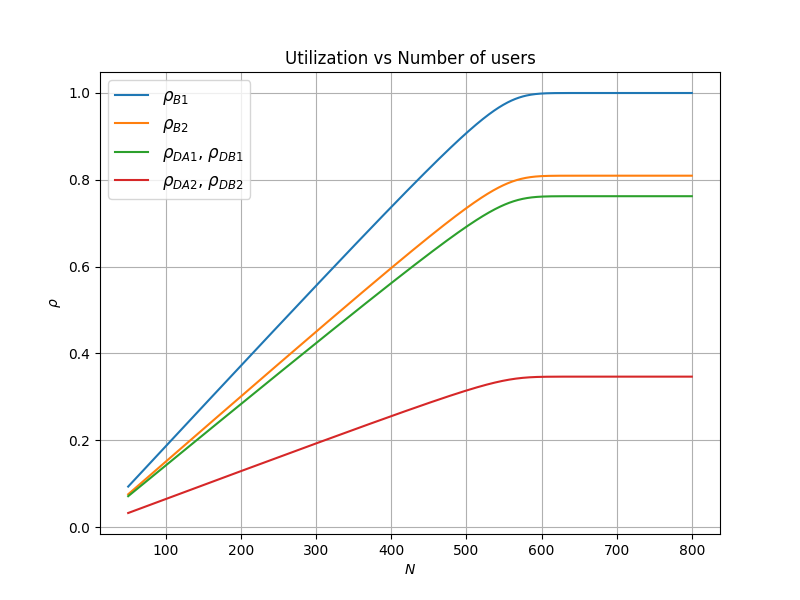
\includegraphics[width=\linewidth]{006/stations-utilization.png}
	\caption{Stations utilisation over the number of users}
\end{figure}

\subsection{Asymptotic bounds}

Utilising the identical mathematical models employed previously (\ref{eq:asymptotic-bounds-expected-response-time}; \ref{eq:asymptotic-bounds-throughput}), we proceed to determine the asymptotic limits for throughput and expected response time.

\[
 R \geq max\left(\num[round-mode=places, round-precision=5]{0.00756138888888889},\;N\times\num[round-mode=places, round-precision=5]{0.00187777777777778}-1\right) \\
\]

\[
 X \leq min\left(\frac{N}{\num[round-mode=places, round-precision=5]{0.00756138888888889}+1},\;\frac{1}{\num[round-mode=places, round-precision=5]{0.00187777777777778}}\right) \\
\]

\subsection{Mean Value Analysis}

Once more, utilising the JMVA software, we proceed to estimate the performance indices of our queueing network and subsequently present the outcomes of the simulation below.

\begin{figure}[h]
	\centering
	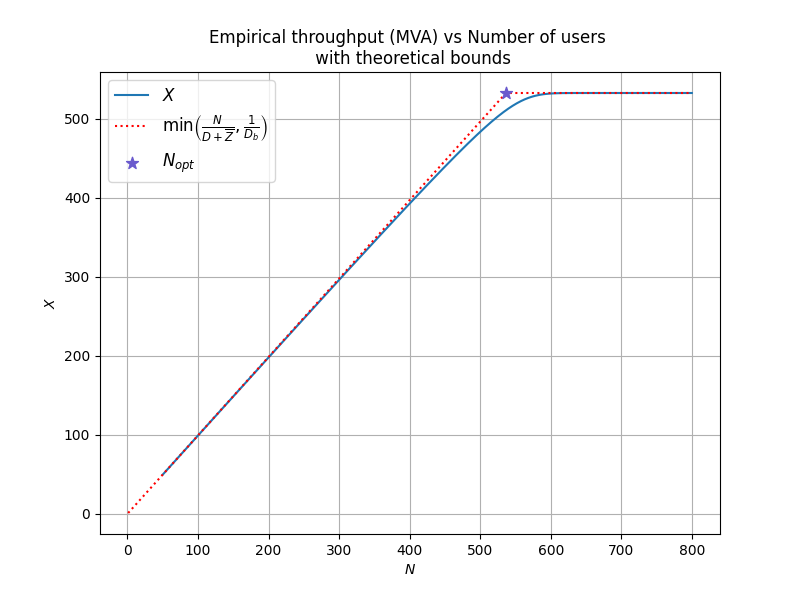
\includegraphics[width=\linewidth]{006/mva-x.png}
	\caption{MVA -- Throughput over the number of users}
\end{figure}

\clearpage

\begin{figure}[h]
	\centering
	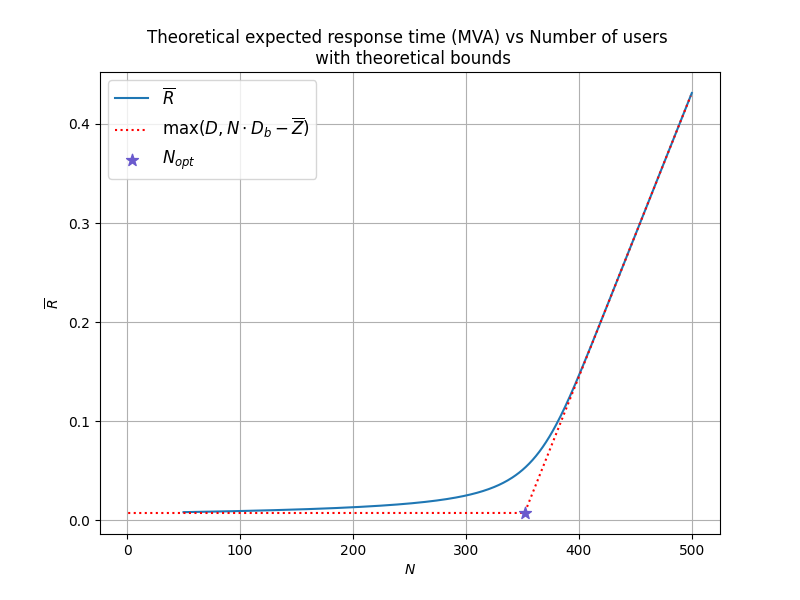
\includegraphics[width=\linewidth]{006/mva-r.png}
	\caption{MVA -- Expected response time over the number of users}
\end{figure}

\subsection{Optimal -- theoretical -- number of users}

In conclusion to the theoretical analysis of the enhanced queuing network, we proceed with the estimation of the optimal number of users by means of the same formula previously adopted. \ref{eq:optimal-number-of-users}

\begin{equation}
	N_{opt} = \frac{\overline{D} + \overline{Z}}{\overline{D}_b} = \num[round-mode=places, round-precision=5]{536.571153846154}
\end{equation}

This result clearly demonstrates that the proposed architecture exhibits superior scalability, enabling an increase of over 180 in the number of optimally manageable users.
